\section{Limitations of Regularized Undirected Exploration }
\label{sec:limitations}
Naturally, how well we can recover the optimal policies depends on the quality of data used to learn them.  However, when $d$ is finite and when the dataset has narrow data distributions, the learning objective lacks sufficient inductive bias on which policies to favor. This often leads to a collapse of the FB representations.

 Consistent with empirical observations in \citep{tirinzoni2025zeroshot}, our findings demonstrate this failure mode. In \Cref{fig:motivation_method} we report the average zero-shot performance when using an \textit{undirected} exploration strategy, i.e., exploring by uniformly sampling random reward embeddings from the hypersphere. We observe that this strategy suffers from performance degradation and entropy stagnation. Additionally, the recovered policies exhibit severe foot dragging which prevents seamless sim-to-real transfer. To mitigate these issues, we propose to ground the unsupervised policy learning by adding a regularizer. Formally, this leads to the actor loss objective:
\begin{equation}
\mathcal{L}_{\text{FB-Critic}}(\pi)
=
-\mathbb{E}_{z\sim\nu,\; s\sim\rho,\; a\sim\pi_z(s)}\Big[
F(s,a,z)^\top z
+
\lambda_{\text{reg}}\,
Q_{\text{reg}}(s,a)
\Big]
\label{eq:actor_loss_with_reg}
\end{equation}
where $Q_\text{reg}$ is a critic trained with a behavior regularizer reward. We refer interested readers to the details at \Cref{appendix:regularization_reward,appendix:qregu}. While this modification regularizes the solution manifold by effectively suppressing foot dragging (see \Cref{fig:motivation_method} (right)), we find that exploration degrades further, resulting in lower entropy and performance.
%leads to overconservative behaviors, severely shrinking the support of the data distribution and resulting in degraded average performance.
To tackle this issues, in the next section we introduce \method, an algorithmic modification to FB exploration strategies to improve downstream task performance.


\begin{figure}[H]
    \centering
    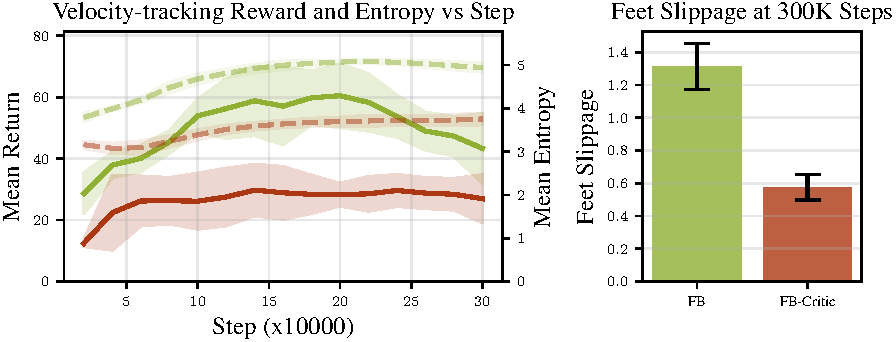
\includegraphics[width=0.8\linewidth]{figure/locomotion_fb_fb_critic.pdf}
   

    % Legend
    \centering
    \minipage{\linewidth}
    \small
    \centering
    \textcolor{ourgreen}{\rule[2pt]{20pt}{3pt}} \textrm{FB} \quad
    \textcolor{ourdarkred}{\rule[2pt]{20pt}{3pt}} \textrm{\algo{FB-Critic}}\quad
    % \textcolor{ourorange}{\hdashrule[2pt]{20pt}{3pt}{2pt 2pt}}\textrm{\algo{dashed example}}
    \endminipage\
    \caption{Limitations of undirected exploration: Standard FB algorithm with undirected exploration (FB) suffers from performance degradation and entropy stagnation (left, higher is better) and yields unnatural behaviors (right, lower is better). While introducing a behavior regularizer (FB-critic) leads to more plausible behaviors (right), it leads to severe performance degradation and further reduces behavior diversity (left).}
    \label{fig:motivation_method}
\end{figure}

\section{Maximum Entropy Behavior Exploration}

\begin{figure}[t]
    \centering
    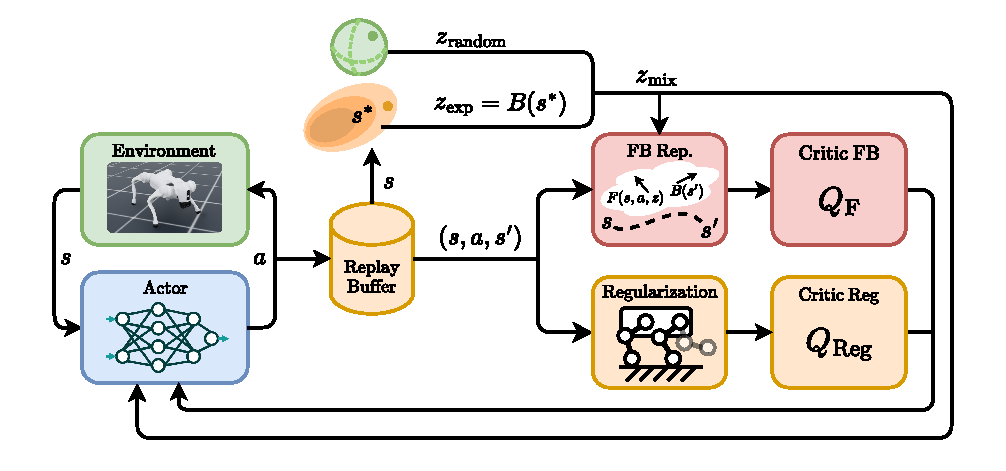
\includegraphics[width=\linewidth]{figure/pipeline.pdf}
    \caption{Maximum Entropy Behavior Forward-Backward Exploration:  \method is an online zero-shot RL algorithm that collects data by acting with behaviors $z_{exp}$ that maximize the entropy of the achieved behavior distribution. Collected data is used to train policies with a regularized loss combining policy improvement objective based on the FB action value function ($Q_{FB}$) and a critic ($Q_{reg}$) trained on a behavior regularizer reward to induce meaningful locomotion patterns.}
    \label{fig:fig_method}
\end{figure}


\subsection{Density-Inverse Exploration for Online FB}


\textit{How should a zero-shot RL agent explore in an environment in order to accumulate diverse, relevant data, while aligned with downstream task of interest?} While we lack a proper characterization of which data is relevant \textit{a priori}, the support of the empirical training distribution $\rho$ must cover the occupancy measures of policies optimal for downstream tasks $z^d_r$. Hence, an exploration strategy should select intrinsic behaviors $z_r^t$ to bring the agent's historical achieved behavior distribution $p^t_{z^a_r}$ close to the downstream behavior distribution $p_{z^d_r}$. This can be formalized with the following distribution matching objective:
\begin{equation}
\label{eq:oracle_loss}
    J_{\text{oracle}}(p^t_{z^a_r}) = D_{KL}(p_{z^d_r} \vert \vert p^t_{z^a_r})
\end{equation}
where $p^t_{z^a_r}$ is the distribution of achieved behaviors in the replay buffer at time $t$ and $D_{KL}$ is the forward KL divergence (support covering).
Unfortunately, in the unsupervised setting, objective in \Cref{eq:oracle_loss} is intractable, because we do not have access to the desired behavior distribution $p_{z^d_r}$. In the absence of a useful inductive bias on the direction where to expand the support of $p_{z^a_r}$, similarly to \citet{pitis2020maximum}, we expand the support on all directions maximizing the entropy of the achieved behavior distribution $H[p^t_{z^a_r}]$. This leads to the following objective:
\begin{equation}
\label{eq:entropy_loss}
    J_{\text{MEBE}}(p^t_{z^a_r}) = -H[p^t_{z^a_r}],
\end{equation}
implicitly inducing a curriculum on the behaviors with which explore next to effectively push the frontier of achievable behaviors. 
% \subsection{Setting intrinsic exploration behaviors}
To optimize \Cref{eq:entropy_loss}, at time $t$ we act with an exploration policy $\pi_t^E$ %which is going to collect data such that the expected entropy of the updated achieved behavior distribution is maximized. Formally, we act with the policy 
with reward embedding $z_r^{E}$ such that
% $z_r^E \sim \nu_{\tiny{\method}}$
\begin{equation}
\label{eq:z_mebe}
    z_r^{E} = \argmax_{z_{r} \in \gZ}\mathbb{E}_{z'_r \sim q(z'_r \vert z_r)} H\big[p^t_{z^a_r \cup z'_r}\big].
\end{equation} 
Importantly, \Cref{eq:z_mebe} depends on $q(z'_r \vert z_r)$ which encodes the conditional probability of achieving behavior $z_r'$ if we act with the policy parameterized with $z_r$, which we do not know. However, we observe that the entropy $H[p^t_{z^a_r}]$ is maximized when the distribution of achieved behaviors is uniform over the behavior space. Consequently, rather than predicting future outcomes, \method steers the achieved behavior distribution towards uniformity by sampling exploration behaviors $z_r^E$ that have the minimum density in the current buffer.%Hence, we select exploration behaviors $z_r^E$ that have minimum density in the current buffer. 

\subsection{Pratical FB-MEBE}
Let $q_\Psi(z^a_r)$ be the density model trained on the achieved behaviors stored in the replay buffer. We sample exploration behaviors according to a distribution that is inversely proportional to their estimated density, i.e., 
\begin{equation}
\label{eq:sample_inv}
   z_r^E \propto ({q}_\psi(z^a_r) + \epsilon)^{-\beta}
\end{equation}
where $\epsilon > 0$ ensures numerical stability and $\beta \ge 0$ controls the strength of the inverse reweighting. 
% This strategy approximates the maximization of the state distribution entropy $H(P(s))$, effectively mitigating occupancy bias during online training.
In practice, because we have direct access to states, we learn the density model on the space of achieved states $q_\Psi(s)$ instead (or on a projection $\varphi(s)$\footnote{To focus exploration on relevant parts of the state space, we learn the density on projections of it i.e., $\varphi: S \rightarrow S'$, where $S\subseteq\sR^d, S' \subseteq \sR^{m}, m<d$.} of it). This effectively focuses on goal-reaching behaviors, i.e., $z_r=B(s)$, and could circumvent challenges arising from representation drifts that occur due to $B$ representations changing through time. 
% An in-depth analysis is left for future work.




 Various approaches can be used to estimate the state density, such as Kernel Density Estimation (KDE), Variational Autoencoders (VAE) \citep{kingma2013auto}, k-NN particle estimators, Random Network Distillation (RND) \citep{rnd} or normalizing flows \citep{rezende2015variational}. We chose normalizing flows (NFs) to fit our density $q_\Psi(s)$ over all the alternatives due to its efficient likelihood evaluation, compared to quadratic computation cost of non-parametric models, while offering true density estimates compared to surrogates produced by RND or VAE. Leveraging NFs for unsupervised goal sampling has been also explored in \citep{normalizing-flow-rl}. Note that during the inverse sampling process, the state $s$ is sampled from the replay buffer rather than from the flow model to improve training stability. Details for the NF can be found in \Cref{tab:nf_hyperparameters}. Finally, we explore with the set of policies with reward embedding
\begin{equation}
\label{eq:practical_fb_mebe}
\{z_j^E = B(s_j^E)\}_{j=1}^K,  \quad s_j^E \sim ({q}^t_\psi(s))^{-\beta}
\end{equation}
where $K$ is the number of exploration policies collecting data in parallel and ${q}^t_\psi(s)$ is the density model fitted on data from the replay buffer at episode $t$. 


Finally, as reported in \Cref{sec:limitations}, \method regularizes exploration by enforcing relevant gait patterns via a behavior regularizer, as in \Cref{eq:actor_loss_with_reg}. 
We provide a pseudocode for our algorithm in \Cref{algo:fb-mebe} and a visual schematic of \method in \Cref{fig:fig_method}. For details, see \Cref{appendix:hyperparams,appendix:qregu}.








\begin{algorithm}
\caption{Maximum entropy behavior exploration (\method)}\label{algo:fb-mebe}
\begin{algorithmic}[1]
    \STATE \textbf{Input:} $F_{\theta}$ and $\bar{F}_{\theta}$, $B_\phi$ and $\bar{B}_{\phi}$, $q_\Psi$, $Q_\mathrm{reg}$ 
    \WHILE{not converged}
        \STATE Sample behavior $z_r^E$ according to \cref{eq:practical_fb_mebe}.
        \STATE Collect data $\gD_n =\mathrm{Rollout}(\pi(z_r^E))$.
        \STATE Add data to buffer $\gD_{1:n} = \gD_{1:n-1} \cup \gD_n$.
        \STATE Fit $F_\theta$, $B_\phi$, policies $\pi_z$, $q_\Psi$ and $Q_\mathrm{reg}$  with $\gD_{1:n}$.
    \ENDWHILE
\end{algorithmic}
\end{algorithm}